\documentclass[10pt]{article}
\usepackage{icmlko}

\icmlmeta{IP 파운데이션 월드모델}{142}{오래된 것이 더 잘 맞으면 나중에 쓴 것이다}{노트 141이 만든 시점 규칙을 내 분류에 대 봤다 --- ``정적''이라 적어 둔 축이 한 도메인에서만 사후였고, 그것을 알아채는 방법이 남았다}

\begin{document}

\twocolumn[
\icmlheader

\begin{abstract}
노트 141이 누수의 세 번째 층으로 \emph{측정 시점}을 세우고 축마다 사전 ·
사후 · 정적을 적었다. 설명문 임베딩과 표지 특징은 ``정적''으로 분류했는데,
그 근거가 ``작품의 성질이니까''라는 짐작이었다. \textbf{짐작을 검정할
방법이 필요했다} --- 수집 과정을 몰라도 자료만으로 사후인지 알 수 있나.
있다. 설명문이 출시 시점에 고정이면 작품 나이와 상관 세기가 무관해야 하고,
계속 갱신되면 오래된 작품일수록 ``지금까지의 성공''이 설명문에 스며들어
상관이 세진다. 도메인마다 후행을 반으로 갈라 쟀다. \textbf{모바일만
걸렸다} --- 오래된 절반의 $|\rho|$ 평균이 0.224, 최근 절반이 0.129로
차가 $+$0.095다. 나머지 일곱은 전부 $\pm$0.02 안이다. 앱스토어 설명과
스크린샷은 계속 갱신되고, 애니 시놉시스 · 책 소개 · 펀딩 페이지는 안
바뀐다. \textbf{그래서 시점은 축의 성질이 아니라 (축, 도메인)의 성질이다.}
그렇게 등록하고 가드를 고쳤다 --- 고치는 길에 하나 더 잡았다. 처음 가드는
축 \emph{이름}을 봤는데, 하네스가 축 이름을 모든 도메인에 붙이고 없는 곳은
마스크 0으로 두므로 값이 없는 도메인까지 걸렸다. \textbf{관측 여부를 봐야
한다.} 마지막으로 이 규칙이 푼 채택을 재 봤다. 글·그림 축을 모바일만 빼고
붙이면 판이 $+$0.4328에서 $+$0.4354로 오르고 전부 붙이면 $+$0.4295로
내린다. \textbf{방향은 맞지만 $+$0.0026은 탐지 한계 아래다} --- 채택이
아니라 규칙의 방향 확인으로만 적는다.
\end{abstract}
]

\begin{figure*}[t]
\centering
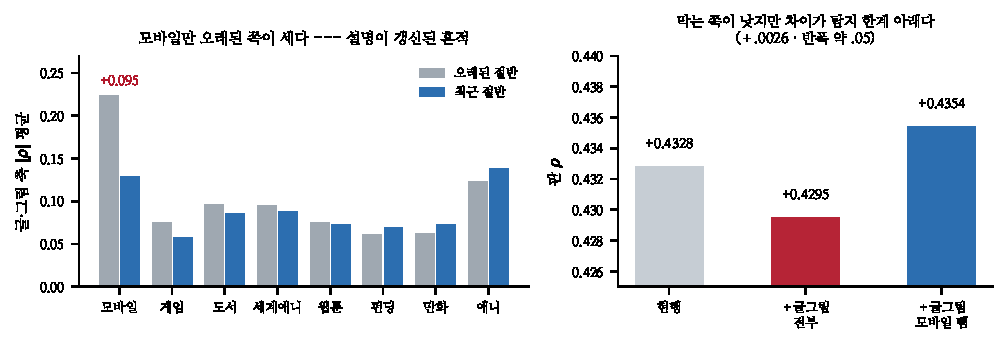
\includegraphics[width=\textwidth]{figs/age.pdf}
\caption{왼쪽 --- 모바일만 오래된 쪽이 세다. 오른쪽 --- 막는 쪽이 낫지만
차이가 탐지 한계 아래다.}
\end{figure*}

\section{짐작을 검정할 방법}

노트 141의 등록부에서 설명문 임베딩 여덟 · 글 특징 다섯 · 표지 특징 일곱을
``정적''으로 적었다. 근거는 ``작품의 성질이니 시간과 무관하다''였는데,
그건 짐작이다. 실제로 그 값들은 \emph{어제} 긁은 스냅샷이다.

수집 과정을 몰라도 자료만으로 알 수 있는 방법이 하나 있다.

\claimx{\textbf{설명문이 고정이면 작품 나이와 상관 세기가 무관해야 한다.}
계속 갱신되면 오래된 작품일수록 그동안의 성공이 설명문에 스며든다 ---
``누적 100만 독자'', ``화제의 신작'' 같은 문구가 뒤에 붙는다. 그러면
오래된 쪽에서 상관이 세진다.}{나이와 상관 세기가 얽히는 다른 이유도
있다 --- 오래된 작품은 라벨이 더 쌓여 잡음이 적다. 그 효과도 같은 방향이라
이 검정은 상한이다.}

\begin{table}[t]
\centering\tsize
\caption{글·그림 축 스무 개의 $|\rho|$ 평균. 후행을 나이로 반 갈랐다.}
\begin{tabular}{lrrr}
\toprule
& 오래된 절반 & 최근 절반 & 차 \\
\midrule
\textbf{모바일} & \textbf{.224} & \textbf{.129} & \textbf{$+$.095} \\
게임 & .075 & .058 & $+$.017 \\
도서 & .097 & .085 & $+$.011 \\
세계애니 & .095 & .088 & $+$.007 \\
웹툰 & .075 & .073 & $+$.002 \\
펀딩 & .061 & .069 & $-$.008 \\
만화 & .062 & .073 & $-$.012 \\
애니 & .123 & .138 & $-$.015 \\
\bottomrule
\end{tabular}
\end{table}

\claimx{\textbf{모바일만 걸린다.} 차가 $+$0.095이고 나머지 일곱은 $\pm$0.02
안이다. 앱스토어 목록은 업데이트마다 설명과 스크린샷이 바뀌고, 애니
시놉시스 · 책 소개 · 펀딩 페이지는 공개 시점에 고정된다.}{여덟 도메인의
관측이다. 웹툰은 $+$0.002로 깨끗한데, 네이버 웹툰 소개글도 갱신될 수
있으니 갱신 폭이 작았을 뿐일 수 있다.}

\section{시점은 (축, 도메인)의 성질이다}

노트 141의 등록부는 축마다 시점을 적었다. 같은 \texttt{emb0}이 애니에서는
정적이고 모바일에서는 사후라면 그 구조로는 못 담는다. 예외를 도메인 단위로
넣었다.

\claimx{\textbf{그리고 가드가 이름을 보고 있었다.} \texttt{harness.load}는
축 이름을 \emph{모든} 도메인에 붙이고 값이 없는 곳은 중립 0.5 · 마스크
0으로 둔다. 이름만 보고 판정하니 ``모바일에서 뺀'' 판도 모바일이 걸렸다.
\textbf{관측 여부를 봐야 한다} --- 마스크 평균이 0에 가까우면 그 도메인은
그 축을 안 쓴다.}{노트 133에서 같은 설계 때문에 한 번 속았다(넓힌 팝업에
축이 안 붙은 것을 한참 못 봤다). \textbf{이름과 값이 갈리는 자리가
반복해서 문제를 만든다.}}

\section{규칙이 푼 채택 --- 방향은 맞고 크기는 없다}

시점 규칙이 정리되면 글·그림 축을 일곱 도메인에서는 쓸 수 있다. 노트
116에서 만들어 놓고 한 번도 안 채택한 축들이다.

\begin{table}[t]
\centering\tsize
\caption{F8 부스팅 · 검색$+$달력 위에.}
\begin{tabular}{lrrrr}
\toprule
& 판 & 모바일 & 애니 & 세계애니 \\
\midrule
현행 & $+$.4328 & $+$.5513 & $+$.4868 & $+$.4933 \\
$+$글그림 전부 & $+$.4295 & $+$.5653 & $+$.4796 & $+$.4633 \\
$+$글그림 모바일 뺌 & \textbf{$+$.4354} & $+$.5462 & $+$.4968 & $+$.4689 \\
\bottomrule
\end{tabular}
\end{table}

\claimx{\textbf{막는 쪽이 낫지만 크기가 없다.} 모바일을 빼면 $+$0.4354,
전부 붙이면 $+$0.4295로 규칙이 가리키는 방향이 맞다. 그런데 현행 대비
$+$0.0026은 판의 탐지 한계 아래다. \textbf{채택이 아니다.}}{전부 붙였을
때 모바일이 $+$0.5513에서 $+$0.5653으로 오르는 것이 눈에 띈다 --- 사후
정보를 쓰면 그 도메인은 좋아 보인다. 규칙이 없으면 그것을 이득으로 읽었을
것이다.}

\section{남긴 것}

\begin{table}[t]
\centering\tsize
\caption{누수 가드 세 층과 검정 방법.}
\begin{tabular}{lll}
\toprule
& 막는 것 & 어떻게 아나 \\
\midrule
① & 라벨의 복사본 & 상관 $\ge$ .70 \\
② & 라벨을 만든 계수기 & 출처 목록 \\
③ & 나중에 잰 것 & 등록부 $+$ \textbf{나이 검정} \\
\bottomrule
\end{tabular}
\end{table}

셋째 줄의 ``나이 검정''이 이 노트가 남기는 것이다. 등록부는 손으로 적으니
빠뜨릴 수 있고, 실제로 노트 141에서 스무 축을 통째로 잘못 적었다. 나이
검정은 자료만으로 그것을 잡는다.

\begin{table}[t]
\centering\tsize
\caption{남은 것.}
\begin{tabular}{ll}
\toprule
나이 검정 & 라벨 누적 효과와 안 갈린다 --- 상한이다 \\
웹툰 & $+$.002 지만 소개글이 갱신될 수 있다 \\
팝업 & 기획서는 사전 문서라 이 문제가 없다 \\
\bottomrule
\end{tabular}
\end{table}

마지막 줄이 위안이다. 팝업의 축은 \emph{사전 문서}에서 매긴 것이라 시점
문제가 원천적으로 없다. 이 프로젝트에서 유일하게 그 성질을 가진 자료이고,
표본이 제일 작은 것도 같은 이유다 --- 사전 문서가 남아 있는 건이 그만큼
드물다.

\end{document}
